% ============================================================
% BRAVE Childcare -- Joypad Control Diagram
%
% Generates a labeled callout diagram by overlaying TikZ
% annotations on a base image of the controller.
%
% HOW TO USE
% ----------
% 1. Compile this file with pdflatex (or lualatex/xelatex):
%       pdflatex GameControls_JoyPad_Diagram.tex
%
% 2. The base image is read from the same directory as this file:
%       GameControls_JoyPad.png
%    Copy (or symlink) the image next to this .tex file if needed.
%
% 3. To re-position a callout, find its ANCHOR COORDINATE in
%    Section 3 and change the (x, y) values.  All coordinates
%    are in centimetres from the lower-left corner of the image.
%    The image is rendered at \imagewidth (default 15 cm).
%
% 4. To move a label box without moving its anchor dot, change
%    the (dx, dy) OFFSET values in Section 4.  The label box is
%    placed at (anchor) + (offset) and connected by a thin line.
%
% 5. To change the label text, edit the third argument of each
%    \joyCallout command in Section 4.
%
% DEPENDENCIES: tikz (with calc, arrows.meta libraries),
%               graphicx, fontenc, inputenc (standard TeX Live)
% ============================================================

\documentclass[border=12pt]{standalone}

\usepackage[T1]{fontenc}
\usepackage[utf8]{inputenc}
\usepackage{graphicx}
\usepackage{tikz}
\usetikzlibrary{calc, arrows.meta}

% ============================================================
% SECTION 1 -- GLOBAL STYLE SETTINGS
%   Tweak fonts, colours, line weight, and box rounding here.
% ============================================================
\tikzset{
  % The small filled circle placed on the controller part
  joyDot/.style={
    circle,
    fill=black!75,
    inner sep=0pt,
    minimum size=5pt
  },
  % The connector line from dot to label box
  joyLine/.style={
    draw=gray!60,
    thick,
    -{Circle[length=4pt, width=4pt, fill=black!75]}
  },
  % The label box
  joyLabel/.style={
    rectangle,
    rounded corners=3pt,
    fill=white,
    draw=gray!50,
    inner xsep=5pt,
    inner ysep=3pt,
    font=\small\sffamily,
    text width=3.0cm,
    align=center,
    text=black
  }
}

% ============================================================
% SECTION 2 -- CALLOUT MACRO
%
%   \joyCallout{<anchor coord>}{<dx,dy offset>}{<label text>}
%
%   <anchor coord>  -- name of a \coordinate defined in Sec. 3
%   <dx,dy offset>  -- relative shift in cm to label box centre
%   <label text>    -- text to display (use \\ for line breaks)
% ============================================================
\newcommand{\joyCallout}[3]{%
  \node[joyDot]  at (#1) {};%
  \draw[joyLine] (#1) -- ++(#2) node[joyLabel] {#3};%
}

\begin{document}
\begin{tikzpicture}

  % ==========================================================
  % SECTION 3 -- BASE IMAGE + ANCHOR COORDINATES
  %
  % The image is placed with its lower-left corner at (0,0).
  % All (x,y) values below are in cm measured from that corner.
  %
  % IMPORTANT: these defaults assume a standard symmetric
  % gamepad photo at 15 cm width.  Adjust every coordinate to
  % match YOUR base image before compiling.
  % ==========================================================

  \def\imagewidth{15cm}   % <-- change if you need a wider/narrower diagram

  \node[anchor=south west, inner sep=0pt] (ctrl) at (0,0)
    {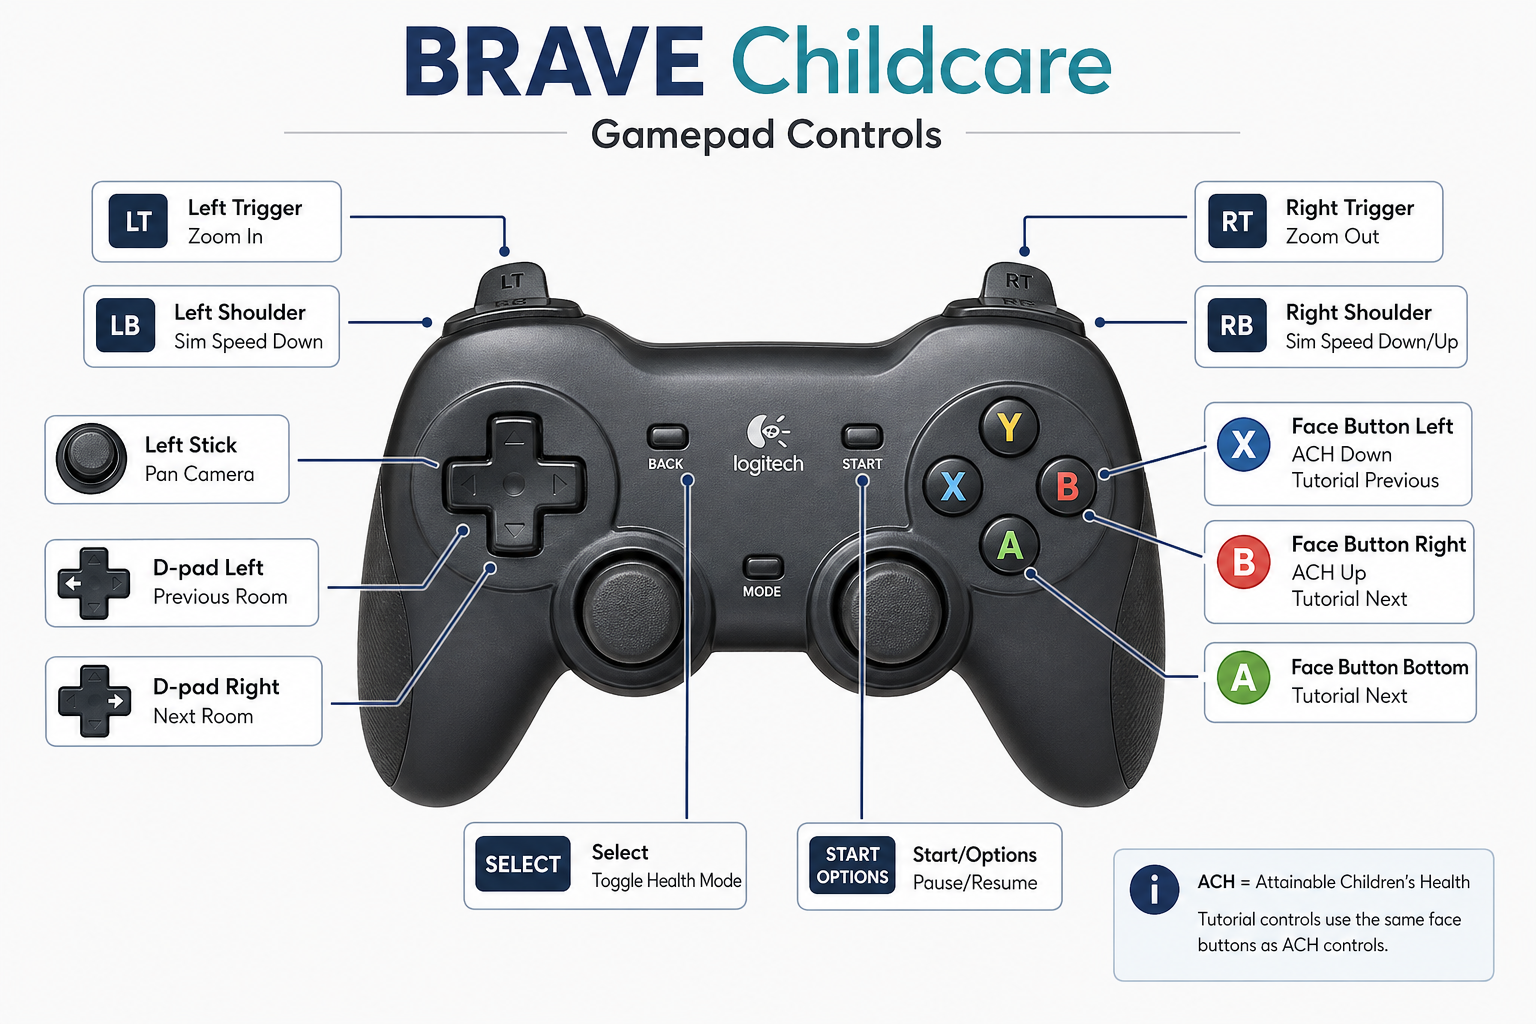
\includegraphics[width=\imagewidth]{GameControls_JoyPad.png}};

  % ---- Left-side controls ----
  \coordinate (leftTrigger)   at (2.2, 7.8);   % Left trigger  (LT / L2)
  \coordinate (leftShoulder)  at (2.8, 6.8);   % Left bumper   (LB / L1)
  \coordinate (leftStick)     at (3.8, 3.8);   % Left analog stick
  \coordinate (dpadLeft)      at (2.4, 4.6);   % D-pad left arrow
  \coordinate (dpadRight)     at (3.6, 4.6);   % D-pad right arrow

  % ---- Centre controls ----
  \coordinate (startBtn)      at (7.5, 5.2);   % Start / Options / Menu button

  % ---- Right-side controls ----
  \coordinate (rightTrigger)  at (12.8, 7.8);  % Right trigger (RT / R2)
  \coordinate (rightShoulder) at (12.2, 6.8);  % Right bumper pair (RB / R1)
  \coordinate (faceLeft)      at (11.0, 5.2);  % Face button left  (X / Square)
  \coordinate (faceBottom)    at (11.8, 4.4);  % Face button bottom (A / Cross)

  % ==========================================================
  % SECTION 4 -- CALLOUTS
  %
  % Each line calls \joyCallout{anchor}{offset}{label}.
  % Offset (dx, dy) is in cm; positive x = right, positive y = up.
  % Increase |dx| to push the label further from the controller.
  % ==========================================================

  % ---- Left-side labels (offset to the left) ----
  \joyCallout{leftTrigger}   {-3.0,  0.8} {Left Trigger\\\textbf{Zoom In}}
  \joyCallout{leftShoulder}  {-3.0,  0.2} {Left Shoulder\\\textbf{Toggle Health Mode}}
  \joyCallout{leftStick}     {-3.2,  0.0} {Left Stick\\\textbf{Pan Camera}}
  \joyCallout{dpadLeft}      {-3.0,  0.8} {D-pad Left\\\textbf{Previous Room} / Tut.\ Prev.}
  \joyCallout{dpadRight}     {-2.8, -0.8} {D-pad Right\\\textbf{Next Room}}

  % ---- Centre label (offset upward) ----
  \joyCallout{startBtn}      { 0.0,  2.2} {Start / Options\\\textbf{Pause / Resume}}

  % ---- Right-side labels (offset to the right) ----
  \joyCallout{rightTrigger}  { 3.0,  0.8} {Right Trigger\\\textbf{Zoom Out}}
  \joyCallout{rightShoulder} { 3.0,  0.2} {Right Shoulder Pair\\\textbf{Sim Speed Down / Up}}
  \joyCallout{faceLeft}      { 3.0,  0.6} {Face Left (X\,/\,$\square$)\\\textbf{ACH Down} / Tut.\ Prev.}
  \joyCallout{faceBottom}    { 3.0, -0.4} {Face Bottom (A\,/\,$\times$)\\\textbf{ACH Up} / Tut.\ Next}

  % ==========================================================
  % SECTION 5 -- FOOTER NOTE
  % ==========================================================
  \node[font=\footnotesize\sffamily\itshape, text=gray!60,
        anchor=north] at (7.5, -0.4)
    {BRAVE Mode toggle is keyboard \texttt{B} by default.};

\end{tikzpicture}
\end{document}
